\chapter{Novel Work}

In this section the work completed so far will be presented. Two main areas of the systematic review process has been focused on. Stopping criteria and indexing/querying pubmed.

\section{Random Sample Method to Stopping}

As approach to determining when to stop looking at document abstracts returned by the query we are proposing a new sampling method. This approach assumes we have optimum ranking algorithm for returning documents for a query.

The first step of this method is to randomly sample a returned set of documents into a subsets. 

\begin{equation}
U = \frac{|D|}{S}
\end{equation}

Where $U$ is the computed randomised subset, $D$ is the document collection and $S$ is the sample size.

We then use this subset $U$ to create a model / baseline for our topic as a way of predicting how many documents one would need to look at to hit a threshold. The intuition behind this approach is that the rate of which relevant documents occur should be relatively similar when the number of returned documents in the same.

A limitation of this sampling method is that for topics with very few documents it is easy for a sample to miss many of them. This creates a subset set bias, where one set contains a larger percentage of relevant documents. Consider a query that returns 10000 candidate documents of which only 10 have been pre-determined to be relevant. Its not too unlikely that a randomly sampled subset would contain 0 relevant documents. We can use the following equation to tell us how much information we can take from a pre-evaluated topic:

\begin{equation}
I = \frac{rel(T_i)}{|T_i|}
\end{equation}

Where $T_i$ is a given topic and $rel$ computes the number of relevant documents for that topic. Therefore $I$ is telling us how useful the topic is at fitting a curve. We can take the average simply by taking the mean of $I$ across all topics:

\begin{equation}
Usefullness = \frac{\sum{I}}{|T|}
\end{equation}



\subsection{Curve Fitting}

Our first approach uses a simple curve fit against a sample set along with a non-linear function. $f(x)$

\begin{equation}
F(x) = n - a\exp^{-kx}
\end{equation}

Where $a$, $k$ and $n$ are learnt weights and $x$ is an associated return rate for a document. We generate the curve using the least squares algorithm \cite{leastsqures}. 

We can visualise the curve along with the confidence intervals. The Y axis is the predicted number of relevant documents for the topic. X axis shows the true number of documents returned for the query. 

\begin{figure}[H]
\center
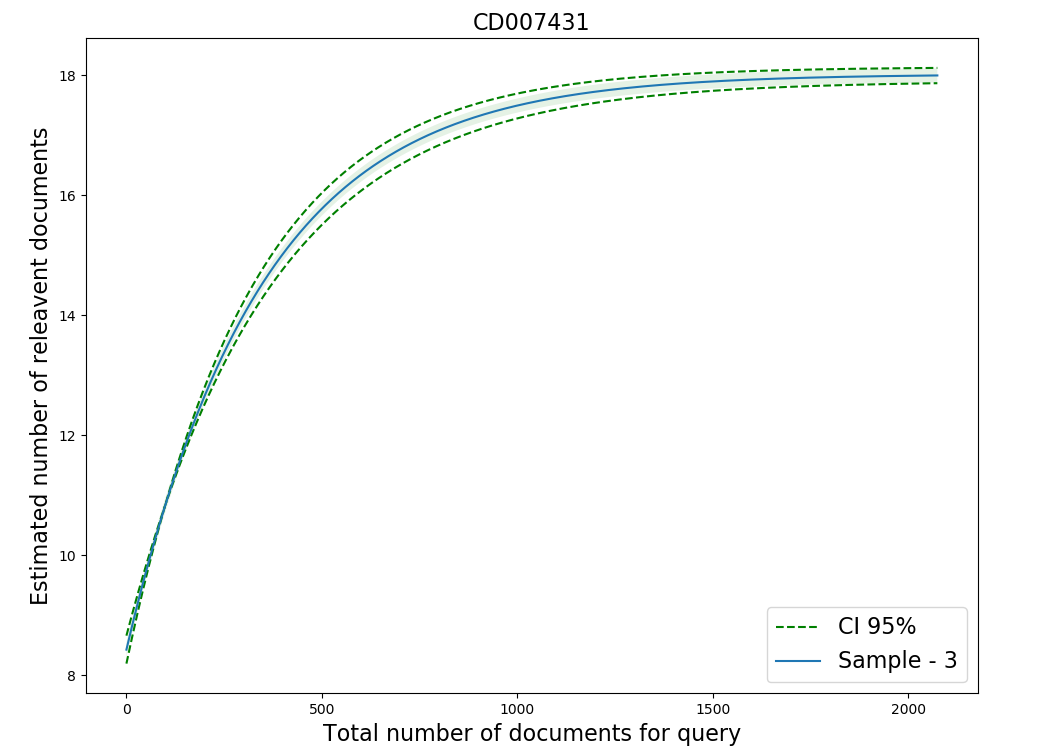
\includegraphics[width=10cm]{figures/curve_fit_example.png}
\caption{Example of fitting a curve for a topic using sampling}
\end{figure}

\begin{table}[H]
\centering
\begin{tabular}{|c|c|c|c|} 

 \hline
 sample size & recall & reliability & effort  \\ 
 1 & 0.91 &	0.96	&	1 \\ 
 3 & 0.66 & 0.5	&	0.48 \\ 
 5 & 0.481 & 0.33	&	0.315 \\ 
 \hline
\end{tabular}
\caption{Comparison of different sample sizes against recall and effort. Ranking Method: Test\_Data\_Sheffield-run-2 \cite{Alharbi2017}}

\end{table}

The first sample size of 1 is included to show how the effort metric is effected. For us to use sample everything, we would need to look at everything, as such the effort averaged out at 1. In this example we were only concerned in achieving 70\% recall, as such even when sampling everything we would really obtain 100\% recall at the expense of 100\% effort.

Looking at every 3rd document and then producing a prediction curve will reduce our effort. We are still required to look at at 1/3 of documents, as such the effort will always be above 0.33. 

\subsubsection{Relevance Ranking}

Our results so far have been based on Test\_Data\_Sheffield-run-2 \cite{Alharbi2017} of CLEF 2017. Naturally, the reliability of our curve is heavily based on how good the initial rankings are for each topic. We can compare different ranking methods for generating our stopping curve. By looking at the CLEF 2017 technology assisted review task \cite{Kanoulas12017} we can determine the best candidates to use.

We also introduce a new column: topics sampled is the number of topics that were evaluated using the curve. This is included as some of the ranking methods do not produce enough relevant documents to generate a suitable curve. 

\begin{table}[H]
\centering
\begin{tabular}{|c|c|c|c|c|} 

 \hline
 Submission & recall & reliability & effort & topics sampled  \\ 
 Test\_Data\_Sheffield-run-2 & 0.66 &	0.5	&	0.48 & 30 \\ 
 Waterloo A-rank-cost & 0.65 & 0.41	&	0.39 & 29 \\ 
 Waterloo B-rank-cost & 0.70 & 0.46	&	0.40 & 30 \\ 
 auth run-1 & 0.71 & 0.5	&	0.41 & 30 \\ 
 auth run-2 & 0.67 & 0.46	&	0.40 & 30 \\ 
 ntu run-1 & 0.56 & 0.18	&	0.54 & 22 \\ 
 ucl full-text & 0.55 & 0.36	&	0.70 & 11 \\ 
 \hline
\end{tabular}
\caption{Comparison of different of sample method using curve fitting for different CLEF 2017 runs. Sample size = 3. Results are taken as averages over all topics for search method. No topic drop-out}

\end{table}


This second set of results will use a mandatory drop out parameter for topics with less than 0.5\% of relevant documents.  The maximum number of topics for this dataset remains at 30.

We also include a confidence interval evaluation for lower bounded range of a $3\sigma$ confidence interval. The key advantages of using a curve as  method of evaluating stopping criteria is being able to make use of this confidence interval in a real systematic review. In the context of a systematic reviewers at the data filtering stage, we could specify that the system is 95\% certain that 70\% of relevant documents have been found. At which point the reviewer can decide if its worth continuing to look at documents.

\begin{figure}[H]
\center
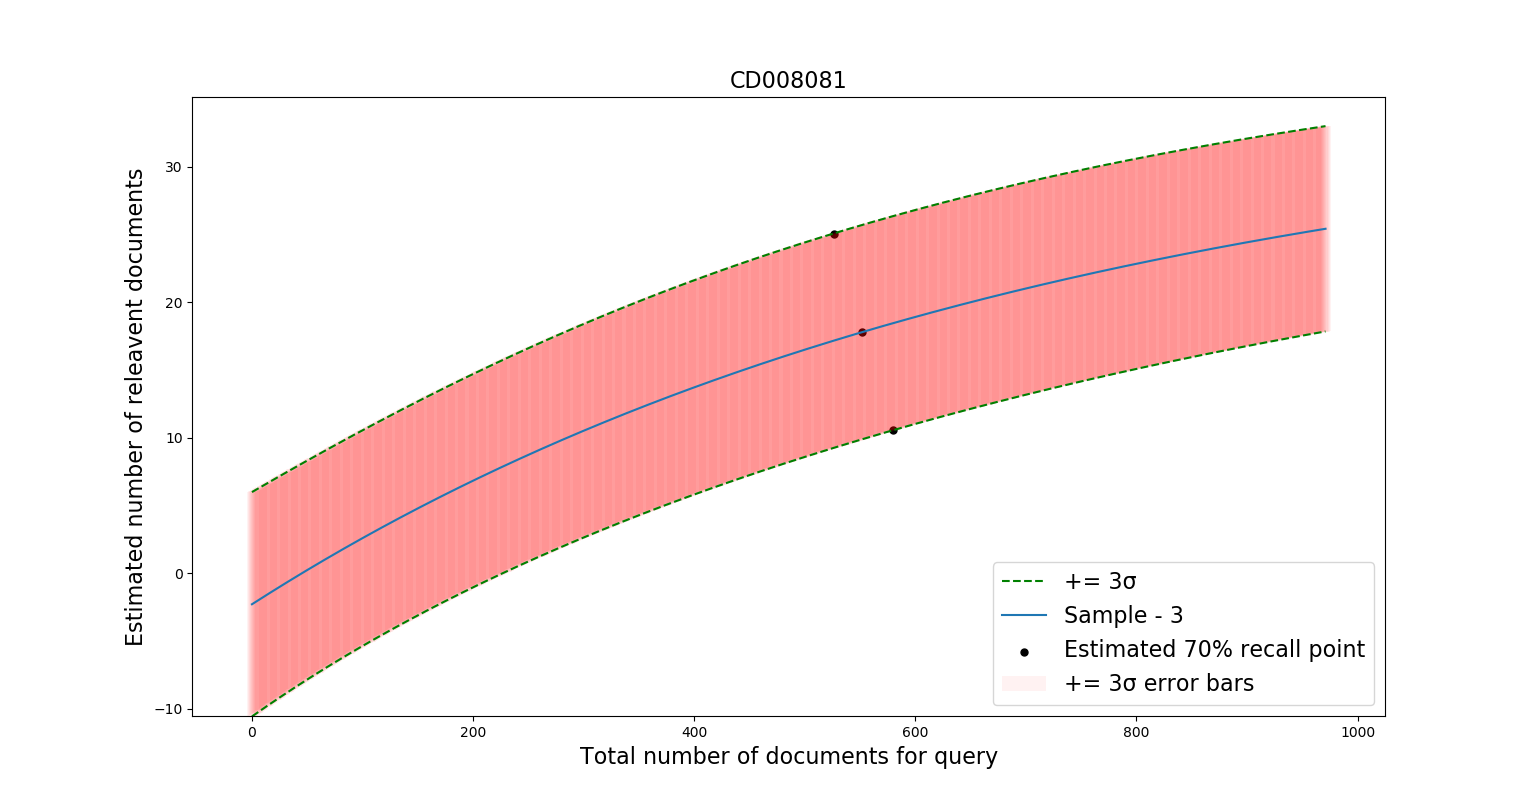
\includegraphics[width=13cm]{figures/cf_example.png}
\caption{Visualisation of using a confidence interval for predicting a stopping point.}
\end{figure}



\begin{table}[H]
\scalebox{0.8}{
\centering
\begin{tabular}{|c|c|c|c|c|} 

 \hline
 Submission & recall-lower & reliability-lower & effort-lower & topics sampled  \\ 
 Test\_Data\_Sheffield-run-2 & 0.70 \, 0.75, &	0.56 \, 0.64	&	0.47 \, 0.51 & 25 \\ 
 Waterloo A-rank-cost & 0.68 \, 0.72, &	0.41 \, 0.45	&	0.40 \, 0.42 & 24 \\ 
 Waterloo B-rank-cost & 0.72 \, 0.758, &	0.53\, 0.80	&	0.41\, 0.42 & 26 \\ 
 auth run-1 & 0.755 \, 0.755, &	0.60 \, 0.60	&	0.42 \, 0.43 & 23 \\ 
 auth run-2 & 0.725 \, 0.757, &	0.54 \, 0.63	&	0.42 \, 0.43 & 22 \\ 
 ntu run-1 & 0.60 \, 0.61, &	0.21 \, 0.28	&	0.53 \, 0.54 & 14 \\ 
 ucl full-text & 0.57 \, 0.60, &	0.33 \, 0.33	&	0.75 \, 0.72 & 6 \\ 
 \hline
\end{tabular}
}
\caption{Comparison of different of sample method using curve fitting for different CLEF 2017 runs. lower = lower-bound confidence interval. Sample size = 3. Results are taken as averages over all topics for search method. with 0.5\% cut-off}

\end{table}

We have deliberately compared two of the better participant rankings (Waterloo and auth) and two of the lower performers (ntu and ucl). We can see the quality of the initial rankings significantly influences the performance of our stopping criteria. This suggests there is a important relationship between using a curve to predict a stopping point and how good the initial ranking of documents is. Some of the ranking methods struggle to produce curves and when combined with a drop-out parameter produce become not worth considering in our evaluation.


\subsection{Gaussian Process fitting}

As an alternate approach to fitting a simple curve, we can apply a GP.

We will apply a constant kernel plus a squared-exponential kernel. One of the key challenges when applying a Gaussian Process was the amount of over-fitting.  




\begin{table}[H]
\scalebox{1.0}{
\centering
\begin{tabular}{|c|c|c|c|c|} 

 \hline
 Submission & recall-lower & reliability-lower & effort-lower & topics sampled  \\ 
 Test\_Data\_Sheffield-run-2 & 0.73 \, 0.73, &	0.73 \, 0.73	&	0.50 \, 0.50 & 26 \\ 
 
 
 Waterloo A-rank-cost & 0.70 \, 0.70, &	0.40 \, 0.40	&	0.42 \, 0.42 & 25 \\ 
 
 
 Waterloo B-rank-cost & 0.73 \, 0.73, &	0.71 \, 0.71	&	0.41 \, 0.41 & 27 \\ 
 
 
 auth run-1 & 0.74 \, 0.75, &	0.56 \, 0.60	&	0.42 \, 0.39 & 23 \\ 
 
 
 auth run-2 & 0.72 \, 0.73, &	0.52 \, 0.52	&	0.42 \, 0.42 & 23 \\ 
 
 
 ntu run-1 & 0.67 \, 0.67, &	0.40 \, 0.40	&	0.64 \, 0.64 & 22 \\ 
 
 
 ucl full-text & 0.72 \, 0.72, &	0.52 \, 0.56	&	0.82 \, 0.82 & 25 \\ 
 \hline
\end{tabular}
}
\caption{Comparison of different of sample method using gp for different CLEF 2017 runs. lower = lower-bound confidence interval. Sample size = 3. Results are taken as averages over all topics for search method. with 0.5\% cut-off}

\end{table}

We can see the gp does a better job at fitting to the topics than the curve method. However, for most of the lower ranking runs the effort is increases significantly, suggesting the gp is not fitting very well to the data.


\begin{figure}[H]
\center
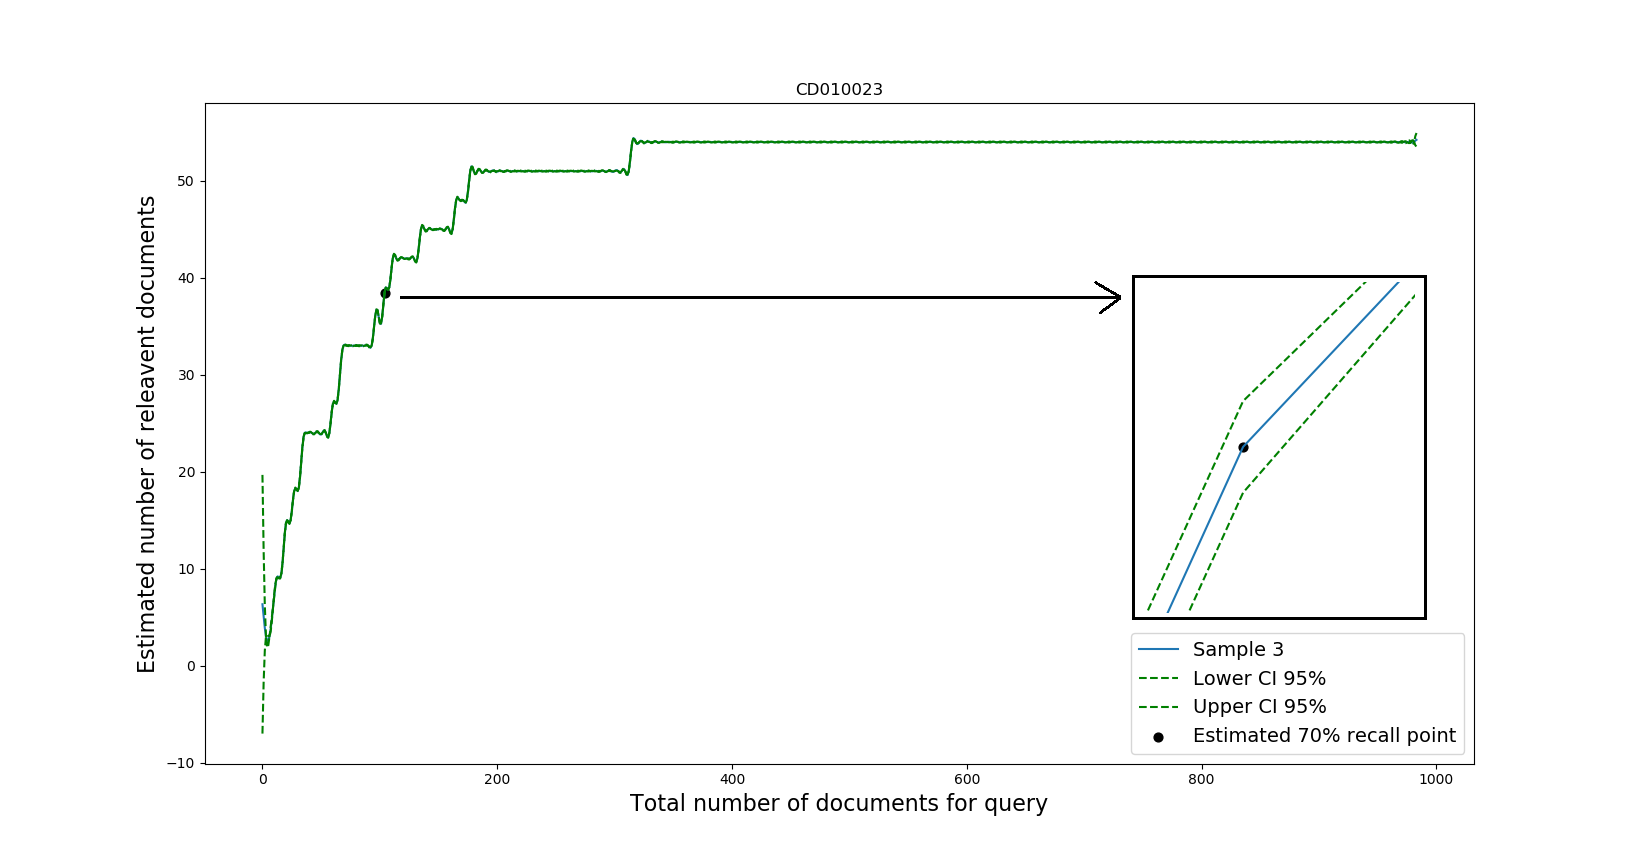
\includegraphics[width=12cm]{figures/joined_graph.png}
\caption{Visualisation of using a confidence interval for predicting a stopping point using a gp. We can see the gp is significantly over fitting to the data.}
\end{figure}


\subsection{Conclusion on Curve fitting and GP}

We implemented two methods for predicting stopping points in ranked medical studies. Our first approach used a general curve to estimate the point in which 70\% recall is likely to have been hit. Our second method used a Gaussian Process in the same way. We used a sampling method to generate our curves to makes predictions about the remaining studies.

\subsubsection{Comparing with Target Method}

\begin{table}[H]

\centering
\begin{tabular}{|c|c|c|c|c|} 
 \hline
 Method & Target & recall & reliability & effort  \\ 

 Target Method & 10 & 0.952 & 0.96 & 0.652 \\
 Sheffield-run2-curve & - & 0.75 & 0.64 & 0.51 \\
 \hline
\end{tabular}
\caption{Comparing target method with curve fitting along with confidence interval. Using Sheffield-run-2}

\end{table}

We can evaluate how well this method does against an existing set of relevance rankings. We will use the Sheffield run data from the CLEF 2017 task \cite{Kanoulas12017}. As the target method allows us to specify our level of reliability, we needed a target $T$ of 9 to hit 95\% reliability. We can see that the reliability of our method does not come close to the Target method. Our curve, however has a much lower effort.

\subsection{Gaussian Process Conclusion}

So far, we found using a GP was not an appropriate choice due to the level of over-fitting. Further work is needed in determining an efficient kernel for our data.


\section{Indexing and Querying Medline using Systematic Review Protocols}

Being able to produce an efficient index of Medline is something highly desirable in the field of medicial research. A more efficient index will produce more concise results when given a query. This could potentially save time in filtering through many non-relevant studies and providing a more concise data-set for reviewers to observe. 

\subsection{Acquiring Key Information from A Systematic Review Protocol}

A systematic review protocol is created before the systematic review process is started. A systematic review protocol describes the rationale, hypothesis, and planned methods of the review. The Medline query is created manually with the help of the protocol. Here we are looking to generate a suitable query/relevant information from the protocol to then automatically query Medline.

We will use RAKE \cite{rake} to extraction key-words from a protocol. The minimum word occurrence count is set to 1, as the protocols are typically small. We used a pubmed stop list as the phrase splitting parameter. Example shown below:

\begin{tcolorbox}

Topic: CD008122 

Title: Rapid diagnostic tests for diagnosing uncomplicated P. falciparum malaria in endemic countries 

Objective: To assess the diagnostic accuracy of RDTs for detecting clinical P. falciparum malaria (symptoms suggestive of malaria plus P. falciparum parasitaemia detectable by microscopy) in persons living in malaria endemic areas who present to ambulatory healthcare facilities with symptoms of malaria, and to identify which types and brands of commercial test best detect clinical P. falciparum malaria.

\end{tcolorbox}

 
\begin{tcolorbox}

endemic countries objective|ambulatory healthcare facilities|rapid diagnostic tests|falciparum parasitaemia detectable|malaria endemic areas|diagnostic accuracy|falciparum malaria

\end{tcolorbox}

The | symbol represents a separation between a phrase. The protcols are pre-processed as follows: Reference removal, lowercase, words less than $N$ length removed, pubmed stoplist. We decided to not perform any stemming/additional manipulation at this stage, due to uncertainty of query format. The resulting content is stored in a separate file appended with '.kwq' (key-word query).

The key-word-query receives some final pre-processing prior to being loaded into our IR system. We used a Lancaster stemmer to reduce words down to a base form. The result is as follows:

\begin{tcolorbox}

endem country object amb healthc facil rapid diagnost test falcipar parasitaem detect malar endem area diagnost acc falcipar malar

\end{tcolorbox}

\subsection{Indexing medline}

Medline was downloaded from the online resource. We processed the xml files and retrieved the  information for each study - title, id, abstract. To reduce the size, we store each record into a local database, containing only the relevant information for each study.

We used Apache Lucene to generate an index for the medline local database. The abstract and title were concatenated together. Pre-processing was done using the same format as the query: pub-med stoplist, Lancaster stemmer and lower casing. 

We will provide comparisons of various ranking methods as well as the evaluation scores for each. 

\subsection{Results}

Results were generated using the eval script from the CLEF 2017/2018 task \cite{Kanoulas12017}. We calculated the top $N$ results over the CLEF 2017 training set. We include a random baseline  to provide a comparison between results.


\begin{table}[H]
\scalebox{0.8}{
\centering
\begin{tabular}{|c|c|c|c|c|c|c|c|} 
 \hline
 Run & recall &  ap & lastrel & wss100 & wss95 & normarea & $N$ \\ 
 Random-baseline & 0.05 &0.02 & 126.7 &0.0 &-0.0 & 0.024 & - \\
 Train-Data-Sheffield-bm25-Run1-objective-only & 0.538 &0.034 & 3039.051 &0.101 &0.108 & 0.431 & 5000 \\
 Train-Data-Sheffield-tfidf-Run1-objective-only & 0.313&0.007& 2633.718&0.021&0.023& 0.247& 5000 \\
 Train-Data-Sheffield-boolean-Run1-objective-only & 0.538 &0.034& 3039.051&0.101 &0.108 & 0.431 & 5000 \\
 Train-Data-Sheffield-bm25-Run1-objective-only & 0.68&0.034& 12310.231&0.169&0.172& 0.592& 25000 \\
 Train-Data-Sheffield-tfidf-Run1-objective-only & 0.601&0.007& 14883.744&0.13&0.136& 0.455& 25000 \\
 Train-Data-Sheffield-boolean-Run1-objective-only & 0.471&0.007& 12974.205&0.03&0.029& 0.381& 25000 \\
 
 \hline
\end{tabular}
}
\caption{Results for IR medline system. Comparison for both 5000 and 25000 thresholds}
\end{table}


As we increase the number of documents we return, the recall naturally increases. When we return 25000 documents for each topic, we are able to obtain a total recall rate of over 58\%. However, the precision (ap, average precision) is very low, suggesting a significant amount of the documents are not useful. BM25 was found to be the best ranking method, followed by tfidf and boolean.

Improvements could certainly be made to this system:

\begin{itemize}
  \item MeSH headings would be useful in expanding the range of the query to capture synonymous terms. 
  \item Tokenization could be optimized to capture phrases of different sizes.
  \item Introducing a cost or stopping point to remove the amount of non-relevant documents. We can see for the 25000 documents set of results the last relevant document was around the 20000 point, meaning we could drop the last 5000 from our result set.
\end{itemize}


\subsection{Medline automatic query Conclusion}


We built an IR system using Apache Lucerne and compared three separate ranking methods. We found bm25 ranking gave the best results overall.

We found we were able to achieve fair results with a little optimization techniques to the index and query data.

We compared the performance of our system across different return thresholds, naturally finding as we increase the returned number of documents we get a higher recall. This comes at the expense of reduced precision.

We suggested further improvement to our system, such as including a phrase model for more robust features for both index and query.



